\chapter{Sistema de reconocimiento de gestos propuesto}\label{capit:cap3}
\vspace{-2.0325ex}%
\noindent
\rule{\textwidth}{0.5pt}
\vspace{-5.5ex}% 
\newcommand{\pushline}{\Indp}% Indent puede ir o no :p 

En este cap\'itulo se describen las etapas del sistema de reconocimiento, junto con los métodos o herramientas que son utilizados en cada una de ellas.   

El sistema de reconocimiento de gestos propuesto consta de cuatro etapas principales. La primera etapa es la adquisición de los datos, en la cual se capturan las imágenes de entrada del sistema; la segunda etapa es la detección, aquí la mano es localizada y segmentada del fondo; en la etapa tres se extraen las características de la mano para ser procesadas; en la etapa final el gesto realizado es reconocido.   
 
  
  
\section{Adquisición de los datos: sensor Kinect}\label{KinectSensor} 

Es la primera etapa del sistema, donde se capturan los datos que son la entrada del sistema. Los datos provienen de los sensores de profundidad de dos dispositivos Kinect. A continuación se describe las características de este dispositivo. 

En noviembre del 2010 la compa\'nia Microsoft lanz\'o el sensor Kinect para consolas de vídeo juego Xbox 360 y en febrero del 2011 lanz\'o la versi\'on para Windows, que se muestra en la figura \ref{fig:KinectPic}.  

El dispositivo Kinect esta equipado con una serie de sensores que permiten obtener imágenes a color y de profundidad (imágenes que indican a la distancia que esta un objeto del sensor), los cuales permiten hacer detección y seguimiento de personas. Detecta $6$ personas y hace el seguimiento de $2$ personas \footnote{https://msdn.microsoft.com/en-us/library/hh973074.aspx}.    
  
\begin{figure}[h!]
\begin{center}
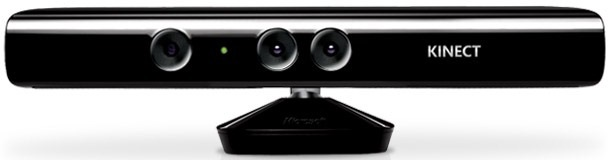
\includegraphics[scale=.6]{./Figures/Kinect.jpg}
\end{center}
\caption{Sensor Kinect para Windows}
\label{fig:KinectPic}
\end{figure} 

El sensor esta equipado con los siguientes componentes: un cámara de color o sensor de color, un emisor infrarrojo, un sensor infrarrojo de profundidad, un motor que controla la inclinación, un arreglo de cuatro micrófonos y un LED \ref{fig:KinectComponentes}. 

\begin{figure}[!h]
\begin{center}
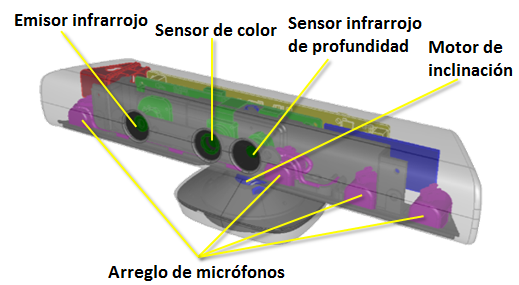
\includegraphics[scale=.6]{./Figures/sensor.png}
\end{center}
\caption{Componentes del sensor Kinect}
\label{fig:KinectComponentes}
\end{figure} 

Enseguida se describen brevemente cada uno de los componentes del sensor Kinect. 
\begin{itemize}
\item La cámara de color captura y transmite datos de vídeo a color, detectando los colores rojo, verde y azul (RGB, por sus siglas en ingl\'es, red, green and blue). La transmisión de datos que brinda la cámara es una secuencia de imágenes (cuadros), a una velocidad de hasta $30$ cuadros por segundo con una resolución de hasta $1280\, x \, 960$ p\'ixeles. La velocidad de los cuadros por segundo varia según la resolución de la imagen.  

\item El emisor infrarrojo proyecta puntos de luz infrarroja frente al sensor, con estos puntos y el sensor de profundidad se puede medir la profundidad que existe del sensor.

\item El sensor infrarrojo lee los puntos infrarrojos proyectados y calcula la distancia que existe entre el objeto y el sensor. El sensor transmite los datos de profundidad con una velocidad de $30$ cuadros por segundo con una resolución de hasta $640 \, x \, 480$ pixeles.   

\item El motor de inclinación controla el \'angulo de la posición vertical de los sensores del dispositivo. El motor puede moverse desde el \'angulo de $-27^ \circ$ a $+27^\circ$. 

\item Arreglo de micrófonos, consta de $4$ micrófonos, captura el sonido y localiza la dirección en la que proviene. 

\item LED indica el estado del sensor.
 
\end{itemize}


 
\section{Detección: detección rápida de objetos usando características simples utilizando el clasificador de cascada impulsada.}\label{sec:ViolaJones}

En esta etapa del sistema el objetivo es localizar y segmentar la mano para extraer las características necesarias para el reconocimiento. 

El m\'etodo  desarrollado por \citep{Viola2001} fue creado originalmente para atacar el problema de detección de rostros, este puede ser usando para detectar cualquier objeto, debido a la forma en que este fue creado, pues detecta un objeto clasificando imágenes basándose en el valor de características simples.

La técnica clasifica si el objeto se encuentra en la escena, usando AdaBoost en forma de cascada, y discrimina el objeto tomando en cuenta el valor de las características, se usan las características Haar, el valor de estas es calculado mediante una imagen integral.

En seguida se explica a detalle cada etapa del método. 

\subsection{Características Haar}\label{subsec:CaracteristicasHaar}  

Las características Haar son operadores rectangulares como los de la figura \ref{fig:haarFeatures}.\\ 
Las características con dos rectángulos \ref{fig:haarFeatures:1}, \ref{fig:haarFeatures:2} , contienen dos regiones rectangulares adyacentes, y el valor de la característica se calcula tomando la diferencia de la suma de ambas regiones.\\ 
Las características con tres rectángulos \ref{fig:haarFeatures:3}, contienen tres regiones rectangulares adyacentes, y el valor de la característica se calcula la suma de las regiones exteriores y se resta la suma de la región interior.\\ 
Las características con cuatro rectángulos \ref{fig:haarFeatures:4}, contienen cuatro regiones rectangulares adyacentes, y el valor de la característica se obtiene con la diferencia entre las regiones pares diagonales.

\begin{figure}%[htbp]
\centering
\subfigure[]{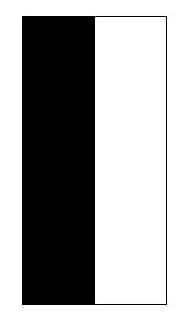
\includegraphics[scale=.4]{./Figures/haarFeatures1}\label{fig:haarFeatures:1}}
\subfigure[]{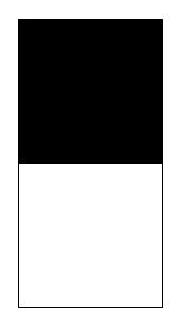
\includegraphics[scale=.4]{./Figures/haarFeatures2}\label{fig:haarFeatures:2}}
\subfigure[]{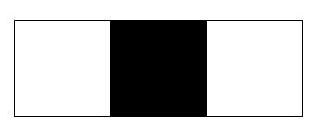
\includegraphics[scale=.4]{./Figures/haarFeatures3}\label{fig:haarFeatures:3}}
\subfigure[]{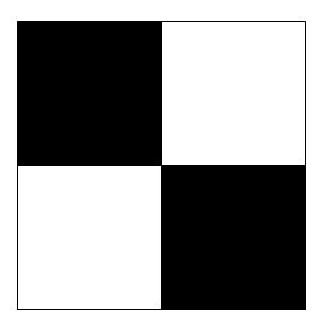
\includegraphics[scale=.4]{./Figures/haarFeatures4}\label{fig:haarFeatures:4}}
\caption{Ejemplo de operadores Haar} \label{fig:haarFeatures}
\end{figure}

\subsection{Imagen integral}\label{subsec:IntegralImage} 

Uno de los aportes de este método es el concepto de imagen integral con la cual se calcula el valor de las características. La imagen integral, $SI$, se calculada como la suma del valor de los pixeles que se encuentran arriba y a la izquierda de cierta posición.    

$$SI(x,y)=S(x,y) + S(x-1,y) + SI(x,y-1)-SI(x-1,y-1)$$ 

La imagen integral permite calcular la suma de los pixeles de cierta región usando solo los valores de las esquinas de dicha región, la cual se obtiene como:   

$$REG(\alpha)=SI(A)+SI(D)-SI(B)-SI(C)$$

donde $REG(\alpha)$ es la región a la cual se le quiere calcular el valor de la suma de sus pixeles; $A,B,C,D$ son las esquinas de dicha región, como se muestra en la figura \ref{fig:figImageIntegral}

\begin{figure}[!h]
\begin{center}
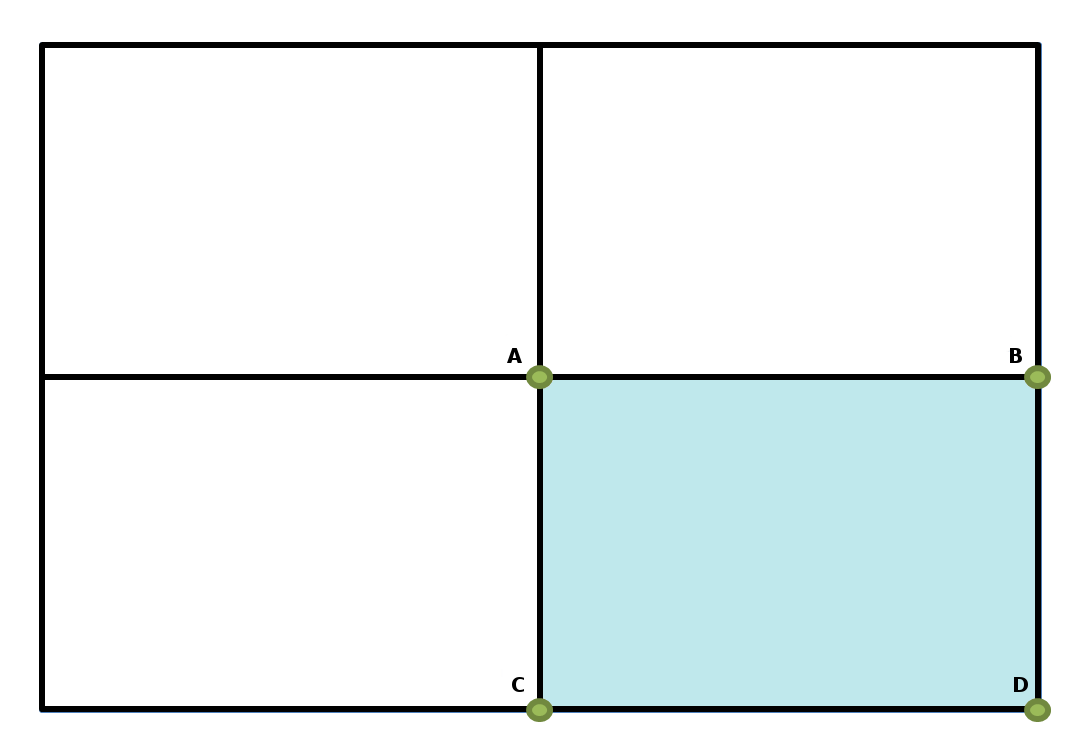
\includegraphics[scale=.3]{./Figures/IntegralImage.png}
\end{center}
\caption{Regiones de imagen integral}
\label{fig:figImageIntegral}
\end{figure} 

\subsection{Clasificador AdaBoost}\label{subsec:AdaboostClasifier}  

El algoritmo AdaBoost realiza su clasificación construyendo un clasificador fuerte $h(x)$ de clasificadores débiles $h_i(x)$. Los clasificares débiles son calculados de la siguiente manera: 

$$h_i(x)=
\begin{cases}   
1, \quad Si \quad  p_if_i<p_i \theta_i \\
0, \quad de \quad otra \quad forma.\\
\end{cases}$$

donde $f_i(x)$ es una característica, $\theta$ es un umbral, y $p_i(x)$ representa el signo de la desigualdad.   

El clasificador fuerte es una combinación lineal de los clasificadores débiles, y se define de la siguiente forma: 

$$h(x)= \alpha_1h_1(x)+\alpha_2h_2(x)+ \cdots +\alpha_nh_n(x)$$ 

donde $n$ es el n\'umero de características, $\alpha_i$ es el valor asociado a cada característica, el cual va entre $0$ y $1$.


\subsection{Clasificador AdaBoost en Cascada}\label{subsec:AdaboostCascade}   


\section{Binarización}\label{Binarization} 

La binarización es una técnica de procesamiento de imágenes, la cual se encarga de transformar una imagen en escala de grises $S(x,y)$ en una imagen binaria $B(x,y)$ es decir, los pixeles de la imagen toman un valor de $0$ ó $1$.   
Para formar la imagen binaria un valor, umbral, de la imagen en escala de grises es seleccionado. Ya que se tiene el umbral, $T$,     
los pixeles de la imagen son discriminados dependiendo si su valor es mayor o igual al umbral entonces el valor de los pixeles en la imagen binaria es $1$ el resto toma valor de $0$. Es decir: 

$$B(x,y)=
\begin{cases}   
1, \quad Si \quad  S(x,y)\geq T \\
0, \quad de \quad otra \quad forma.\\
\end{cases}$$

Existen diversas técnicas para binarizar una imagen, estas se pueden clasificar en dos grupos dependiendo de la manera es que es calcula el umbral, global o local. Los métodos globales calculan un umbral que es usado en toda la imagen y los métodos locales calculan varios umbrales para ciertas regiones de la imagen.  

Un método de binarización muy utilizado es el de NiBlack, \citep{Chaki2014} es un método local y adaptativo ya que adapta el umbral basándose en la media $m(i,j)=$ y la desviación estándar $\sigma(i,j)$ de una ventana deslizante de tamaño $bxb$. El umbral $T$  se calcula como: 

$$T(i,j)=m(i,j)+k \cdot \sigma(i,j)$$ 

donde $k \in [0,1]$ el valor de la constante determina que tanta parte del contorno es preservado.


  
\section{Operaciones Morfológicas}\label{OperacionesMorfologicas} 

Otra técnica muy utilizada en procesamiento de imágenes son las operaciones morfológicas que son un conjunto de operaciones no lineales, la idea es que al aplicar alguna de estas operaciones el ruido se removido tomando en cuanta la forma y estructura de la imagen. 
La operaciones morfológicas utilizan un elemento estructural el cual se aplica por toda la imagen, los elementos estructurales pueden ser de distintas formas como \ref{fig:EX}

\begin{figure}
\centering
\subfigure[Rectángulo de $3x3$.]{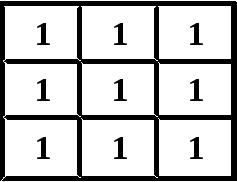
\includegraphics[scale=.7]{./Figures/EX1}\label{fig:EX:1}} %\hspace{20mm}
\qquad
\subfigure[Figura de $3x2$.]{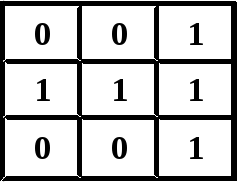
\includegraphics[scale=.7]{./Figures/EX3}\label{fig:EX:3}} 
\\
\subfigure[Cruz de $5x5$.]{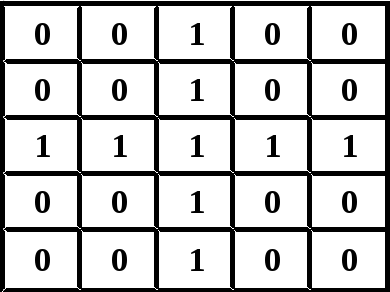
\includegraphics[scale=.7]{./Figures/EX2}\label{fig:EX:2}}
\caption{Ejemplos de elementos estructurales} \label{fig:EX}
\end{figure} 

Existen distintas operaciones morfológicas, las principales o básicas son la dilatación y erosión las cuales se explican enseguida junto con la apertura y el cierra. 
 
\subsection{Dilatación}\label{Dilatation}

La dilatación es una operación que añade pixeles a la orilla de los objetos que se encuentran en la imagen. La dilatación se define como:  
$$S \oplus EX = \lbrace S|EX_S \subseteq S \rbrace$$  
donde $EX_S$ es el elemento estructural trasladado con la imagen. 

\subsection{Erosión}\label{OMerosion}

La erosión remueve pixeles a la orilla de los objetos que se encuentran en la imagen. La erosión se define como: 
$$S \ominus EX = \lbrace S|EX_S \subseteq S \rbrace$$ 
donde $EX_S$ es el elemento estructural trasladado con la imagen. 

\subsection{Apertura}\label{Opening} 

La operación apertura abre huecos entre objetos conectados por un enlace delgado de pixeles.  

$$S \circ EX = (S \ominus EX) \oplus EX $$

\subsection{Cierre}\label{Closure}

La operación cierre elimina huecos pequeños  y rellena huecos en las
$$S \bullet EX = (S \oplus EX) \ominus EX $$

\section{Extracción de características: casco convexo y defectos de convexidad}\label{sec:Convexhull} 

La idea de esta etapa es encontrar las características que sean capaces de describir la mano, de manera que con estas características se pueda reconocer los gestos realizados por la o las manos.  
Las características se guardan en un vector, llamado vector de características, donde la dimension del vector es el número de características que describen, es este caso, la mano.  

Las características que se extraen son geométricas, se extraen: el n\'umero de dedos, los ángulos entre ellos, el centro de la mano, la distancia del centro a la punta de los dedos, el área y perímetro de la mano. 

Antes de definir el casco convexo se presenta la definición de conjunto convexo. 
 

Sea $C$ un conjunto de puntos en el plano Euclidiano, el casco convexo es el conjunto convexo más pequeño que contiene a todos los puntos en $C$. 

Los defectos de convexidad de un con casco convexo, es el conjunto de puntos que no pertenecen al casco convexo. El defecto es el espacio entre la linea y el objeto  



\section{Reconocimiento: m\'aquinas de soporte vectorial}\label{sec:SVM} 
Es la etapa final del reconocimiento,es donde finalmente el gesto puede ser interpretado por la computadora.  

$N$ puntos de entrenamiento de dimensión $D$, dos clases distintas $y_i=-1$
o $+1$ es decir: 

${x_i,y_i}$ donde $i=1, \cdots ,N$, $y\in{-1,1}$, $x \in \Re^D$  

Hiperplano óptimo 
 
$$ w \cdot x + b = 0$$ 

donde $w$ es la normal al hiperplano, $\frac{b}{|w|}$ es la distancia perpendicular desde el hiperplano al origen.   

$$ w \cdot x + b = +1 \textrm{ para } y_i=+1$$ 
$$ w \cdot x + b = -1 \textrm{ para } y_i=-1$$ 

Maximizar el margen, encontrar el mínimo de $w$.  

$Min$ $\Vert w \Vert$ tal que $y_i(w \cdots x_i + b) -1 \geq 0$
 
\begin{figure}[!h]
\begin{center}
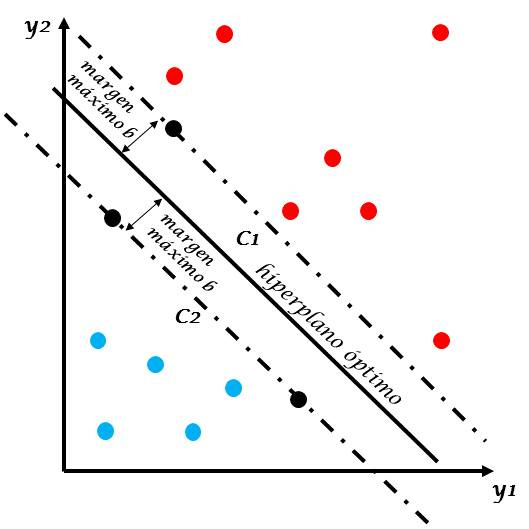
\includegraphics[scale=.3]{./Figures/maquinaSoporte.jpg}
\end{center}
\caption{Clasificación de maquina de soporte usando kernel lineal}
\label{fig:SVM}
\end{figure} 


\newpage
%%=====================================================
